% Options for packages loaded elsewhere
\PassOptionsToPackage{unicode}{hyperref}
\PassOptionsToPackage{hyphens}{url}
%
\documentclass[
  ignorenonframetext,
]{beamer}
\usepackage{pgfpages}
\setbeamertemplate{caption}[numbered]
\setbeamertemplate{caption label separator}{: }
\setbeamercolor{caption name}{fg=normal text.fg}
\beamertemplatenavigationsymbolsempty
% Prevent slide breaks in the middle of a paragraph
\widowpenalties 1 10000
\raggedbottom
\setbeamertemplate{part page}{
  \centering
  \begin{beamercolorbox}[sep=16pt,center]{part title}
    \usebeamerfont{part title}\insertpart\par
  \end{beamercolorbox}
}
\setbeamertemplate{section page}{
  \centering
  \begin{beamercolorbox}[sep=12pt,center]{part title}
    \usebeamerfont{section title}\insertsection\par
  \end{beamercolorbox}
}
\setbeamertemplate{subsection page}{
  \centering
  \begin{beamercolorbox}[sep=8pt,center]{part title}
    \usebeamerfont{subsection title}\insertsubsection\par
  \end{beamercolorbox}
}
\AtBeginPart{
  \frame{\partpage}
}
\AtBeginSection{
  \ifbibliography
  \else
    \frame{\sectionpage}
  \fi
}
\AtBeginSubsection{
  \frame{\subsectionpage}
}
\usepackage{amsmath,amssymb}
\usepackage{iftex}
\ifPDFTeX
  \usepackage[T1]{fontenc}
  \usepackage[utf8]{inputenc}
  \usepackage{textcomp} % provide euro and other symbols
\else % if luatex or xetex
  \usepackage{unicode-math} % this also loads fontspec
  \defaultfontfeatures{Scale=MatchLowercase}
  \defaultfontfeatures[\rmfamily]{Ligatures=TeX,Scale=1}
\fi
\usepackage{lmodern}
\ifPDFTeX\else
  % xetex/luatex font selection
\fi
% Use upquote if available, for straight quotes in verbatim environments
\IfFileExists{upquote.sty}{\usepackage{upquote}}{}
\IfFileExists{microtype.sty}{% use microtype if available
  \usepackage[]{microtype}
  \UseMicrotypeSet[protrusion]{basicmath} % disable protrusion for tt fonts
}{}
\makeatletter
\@ifundefined{KOMAClassName}{% if non-KOMA class
  \IfFileExists{parskip.sty}{%
    \usepackage{parskip}
  }{% else
    \setlength{\parindent}{0pt}
    \setlength{\parskip}{6pt plus 2pt minus 1pt}}
}{% if KOMA class
  \KOMAoptions{parskip=half}}
\makeatother
\usepackage{xcolor}
\newif\ifbibliography
\usepackage{graphicx}
\makeatletter
\def\maxwidth{\ifdim\Gin@nat@width>\linewidth\linewidth\else\Gin@nat@width\fi}
\def\maxheight{\ifdim\Gin@nat@height>\textheight\textheight\else\Gin@nat@height\fi}
\makeatother
% Scale images if necessary, so that they will not overflow the page
% margins by default, and it is still possible to overwrite the defaults
% using explicit options in \includegraphics[width, height, ...]{}
\setkeys{Gin}{width=\maxwidth,height=\maxheight,keepaspectratio}
% Set default figure placement to htbp
\makeatletter
\def\fps@figure{htbp}
\makeatother
\setlength{\emergencystretch}{3em} % prevent overfull lines
\providecommand{\tightlist}{%
  \setlength{\itemsep}{0pt}\setlength{\parskip}{0pt}}
\setcounter{secnumdepth}{-\maxdimen} % remove section numbering
%\usetheme{metropolis}


%\setbeamercolor{normal text}{bg=white}
%\addtobeamertemplate{frametitle}{}{\vspace{-0.5em}} % decrease
%\setbeamersize{text margin left=5mm,text margin right=10mm}
%\usefonttheme[onlymath]{serif}
%\usefonttheme{professionalfonts}
%%%%%%%%%%%%%%%%
% Packages
%%%%%%%%%%%%%%%%

\usepackage{geometry}
\usepackage{graphicx}
\usepackage{amssymb}
\usepackage{amsopn}
\usepackage{cancel}
\usepackage{epstopdf}
\usepackage{amsmath}  	% this permits text in eqnarray among other benefits
\usepackage{url}		% produces hyperlinks
\usepackage{hyperref}	% allows for color usage in tables
\usepackage[english]{babel}
%\usepackage[latin1]{inputenc}
\usepackage{colortbl}	% allows for color usage in tables
\usepackage{multirow}	% allows for rows that span multiple rows in tables
\usepackage{color}		% this package has a variety of color options
\usepackage{xcolor}
\usepackage{pgf}
\usepackage{calc}
\usepackage{ulem}
\usepackage{multicol}
\usepackage{booktabs}
\usepackage{textcomp}
%\usepackage[misc]{ifsym} % for the dice symbol \Cube{}
%\usepackage{txfonts}
%\usepackage{listings}
%\usepackage{tikz}
\usepackage{array}
\usepackage{wasysym}
\usepackage{fancyvrb}

%% change fontsize of R code
\ifdefined\Shaded
\let\oldShaded\Shaded
\let\endoldShaded\endShaded
\renewenvironment{Shaded}{\footnotesize\oldShaded}{\endoldShaded}
\fi
%% change fontsize of output
\let\oldverbatim\verbatim
\let\endoldverbatim\endverbatim
\renewenvironment{verbatim}{\footnotesize\oldverbatim}{\endoldverbatim}

%%%%%%%%%%%%%%%%
% Remove navigation symbols
%%%%%%%%%%%%%%%%

\setbeamertemplate{navigation symbols}{}

\setbeamertemplate{footline}[frame number]

%%%%%%%%%%%%%%%%
% User defined colors
%%%%%%%%%%%%%%%%

\xdefinecolor{oiB}{rgb}{0.22,0.52,0.72}
\definecolor{oiG}{rgb}{.298,.447,.114}
\xdefinecolor{hlblue}{rgb}{0.051,0.65,1}
\xdefinecolor{gray}{rgb}{0.5, 0.5, 0.5}
\xdefinecolor{darkGray}{rgb}{0.3, 0.3, 0.3}
\xdefinecolor{darkerGray}{rgb}{0.2, 0.2, 0.2}
\xdefinecolor{rubineRed}{rgb}{0.89,0,0.30}
\xdefinecolor{irishGreen}{rgb}{0,0.60,0}	
\definecolor{lightGreen}{rgb}{0.387,0.581,0.148}

%%%%%%%%%%%%%%%%
% Template colors
%%%%%%%%%%%%%%%%

%\setbeamercolor*{palette primary}{fg=white,bg= oiB!80!black!90}
%\setbeamercolor*{palette secondary}{fg=black,bg= oiB!80!black}
%\setbeamercolor*{palette tertiary}{fg=white,bg= oiB!80!black!80}
%\setbeamercolor*{palette quaternary}{fg=white,bg= oiB}
%\setbeamercolor{structure}{fg= oiB}
%\setbeamercolor{frametitle}{bg= oiB!90}
%\setbeamertemplate{blocks}[shadow=false]
%\setbeamersize{text margin left=2em,text margin right=2em}

%\setbeamercolor{code body}{bg=gray!20!white!80,fg=black}


%%%%%%%%%%%%%%%%
% Get rid of fancy enumerated list bullets
%%%%%%%%%%%%%%%%

%\setbeamertemplate{enumerate items}[default]

%%%%%%%%%%%%%%%%
% Custom commands
%%%%%%%%%%%%%%%%

\newcommand{\Sum}{\sum\nolimits}
\newcommand{\Hide}[2]{\underline{~~~\onslide<#1>{\alert{#2}}~~~}}
\newcommand{\hide}[2]{\underline{~~\onslide<#1>{\alert{#2}}~~}}
\newcommand{\hid}[2]{\onslide<#1>{\alert{#2}}}
\newcommand{\code}[1]{\textcolor{blue}{\texttt{#1}}}

% red
\newcommand{\red}[1]{\textit{\textcolor{rubineRed}{#1}}}

% pink
\newcommand{\pink}[1]{\textit{\textcolor{rubineRed!90!white!50}{#1}}}

% green
\newcommand{\green}[1]{\textit{\textcolor{irishGreen}{#1}}}

% orange
\newcommand{\orange}[1]{\textit{\textcolor{orange}{#1}}}

% links: webURL, webLin, appLink
\newcommand{\webURL}[1]{\urlstyle{same}{ \textit{\textcolor{darkGray}{\url{#1}}}}}
\newcommand{\webLink}[2]{\href{#1}{\textcolor{darkGray}{{#2}}}}
\newcommand{\appLink}[2]{\href{#1}{\textcolor{white}{{#2}}}}

% mail
\newcommand{\mail}[1]{\href{mailto:#1}{\textit{\textcolor{darkGray}{#1}}}}

% highlighting: hl, hlGr, mathhl
\newcommand{\hl}[1]{\textit{\textcolor{hlblue}{#1}}}
\newcommand{\hlGr}[1]{\textit{\textcolor{lightGreen}{#1}}}
\newcommand{\mathhl}[1]{\textcolor{hlblue}{\ensuremath{#1}}}

% two col: two columns
\newenvironment{twocol}[4]{
\begin{columns}[c]
\column{#1\textwidth}
#3
\column{#2\textwidth}
#4
\end{columns}
}





%%%%%%%%%%%%%%%%
% Change margin
%%%%%%%%%%%%%%%%

\newenvironment{changemargin}[2]{%
\begin{list}{}{%
\setlength{\topsep}{0pt}%
\setlength{\leftmargin}{#1}%
\setlength{\rightmargin}{#2}%
\setlength{\listparindent}{\parindent}%
\setlength{\itemindent}{\parindent}%
\setlength{\parsep}{\parskip}%
}%
\item}{\end{list}}

%%%%%%%%%%%%%%%%
% Footnote
%%%%%%%%%%%%%%%%

\long\def\symbolfootnote[#1]#2{\begingroup%
\def\thefootnote{\fnsymbol{footnote}}\footnote[#1]{#2}\endgroup}

%%%%%%%%%%%%%%%%
% Graphics
%%%%%%%%%%%%%%%%

\DeclareGraphicsRule{.tif}{png}{.png}{`convert #1 `dirname #1`/`basename #1 .tif`.png}



\setbeamercolor{normal text}{bg=white}

\DeclareMathOperator{\var}{var}
\newcommand{\boxmodel}[1]{\begin{array}{|c|}#1\\[2pt]\hline\end{array}}
\newcommand{\BXX}[2]{\begin{array}{|@{\,}c@{\,}|@{\,}c@{\,}|}\hline#1&#2\\[-1pt]\hline\end{array}}
\newcommand{\p}{\mathrm{P}}
\newcommand{\SE}{\mathrm{SE}}
\newcommand{\xbar}{\overline{x}}
\newcommand{\Xbar}{\overline{X}}
\newcommand{\ybar}{\overline{y}}
\newcommand{\Ybar}{\overline{Y}}
\newcommand{\zbar}{\overline{z}}
\newcommand{\Zbar}{\overline{Z}}
\newcommand{\wbar}{\overline{w}}
\newcommand{\Wbar}{\overline{W}}
\newcommand{\vbar}{\overline{v}}
\newcommand{\Vbar}{\overline{V}}
\newcommand{\dbar}{\overline{d}}
\newcommand{\Dbar}{\overline{D}}
\newcommand{\ebar}{\overline{e}}
\newcommand{\ehat}{\widehat{\epsilon}}
\newcommand{\yhat}{\widehat{y}}
\newcommand{\Yhat}{\widehat{Y}}
\newcommand{\bhat}{\widehat{\beta}}
\newcommand{\dl}[1]{\widehat{\delta}_{#1}}
\newcommand{\g}[1]{\widehat{\gamma}_{#1}}
\newcommand{\al}[1]{\widehat{\alpha}_{#1}}
\newcommand{\Bj}{{\beta_j}}
\newcommand{\Bp}{{\beta_p}}
\newcommand{\Bq}{{\beta_q}}
\renewcommand{\b}[1]{\widehat{\beta}_{#1}}
\newcommand{\B}[1]{{\beta}_{#1}}
\newcommand{\BETA}{{\boldsymbol\beta}}
\newcommand{\bp}{\widehat{\beta}_p}
\newcommand{\bq}{\widehat{\beta}_q}
\newcommand{\bj}{\widehat{\beta}_j}
\newcommand{\df}{\mathrm{df}}
\DeclareMathOperator{\VIF}{VIF}
\DeclareMathOperator{\SSE}{SSE}
\DeclareMathOperator{\SST}{SST}
\DeclareMathOperator{\SSR}{SSR}
\DeclareMathOperator{\MSE}{MSE}
\DeclareMathOperator{\MST}{MST}
\DeclareMathOperator{\MSR}{MSR}
\DeclareMathOperator{\RM}{RM}
\DeclareMathOperator{\FM}{FM}
\DeclareMathOperator{\E}{E}
\DeclareMathOperator{\SD}{SD}
\DeclareMathOperator{\se}{se}
\DeclareMathOperator{\cov}{Cov}
\DeclareMathOperator{\corr}{Corr}
\DeclareMathOperator{\cor}{Cor}
\DeclareMathOperator{\Var}{Var}
\DeclareMathOperator{\logit}{logit}
\newcommand{\hsigma}{\widehat{\sigma}}
\newcommand{\betahat}{\widehat{\beta}}
\newcommand{\slide}{<br><br><br><br><br>}
\newcommand{\bbeta}{\boldsymbol{\beta}}
\newcommand{\bX}{\mathbf{X}}
\newcommand{\bY}{\mathbf{Y}}
\newcommand{\bH}{\mathbf{H}}
\newcommand{\bI}{\mathbf{I}}
\newcommand{\be}{\mathbf{e}}
\newcommand{\pval}{\mathit{P}\mathrm{-val}}



\newcommand{\vmu}{\mbox{\boldmath{$\mu$}}}
\newcommand{\vR}{\mbox{\boldmath{$R$}}}
\newcommand{\vpsi}{\mbox{\boldmath{$\psi$}}}
\newcommand{\vZ}{\mbox{\boldmath{$Z$}}}
\newcommand{\vX}{\mbox{\boldmath{$X$}}}
\newcommand{\vY}{\mbox{\boldmath{$Y$}}}
\newcommand{\vW}{\mbox{\boldmath{$W$}}}
\newcommand{\vz}{\mbox{\boldmath{$z$}}}
\newcommand{\vr}{\mbox{\boldmath{$r$}}}
\newcommand{\vx}{\mbox{\boldmath{$x$}}}
\newcommand{\vk}{\mbox{\boldmath{$k$}}}
\newcommand{\vp}{\mbox{\boldmath{$p$}}}
\newcommand{\vv}{\mbox{\boldmath{$v$}}}
\newcommand{\vg}{\mbox{\boldmath{$g$}}}
\newcommand{\vbeta}{\mbox{\boldmath{$\beta$}}}
\newcommand{\vone}{\mbox{\boldmath{$1$}}}
\newcommand{\vep}{\mbox{\boldmath{$\epsilon$}}}
\newcommand{\veta}{\mbox{\boldmath{$\eta$}}}
\newcommand{\vl}{\mbox{\boldmath{$l$}}}
\newcommand{\ve}{\mbox{\boldmath{$e$}}}
\newcommand{\va}{\mbox{\boldmath{$a$}}}
\newcommand{\vb}{\mbox{\boldmath{$b$}}}
\newcommand{\vPsi}{\mbox{\boldmath{$\Psi$}}}
\DeclareMathOperator*{\V}{\mathbb{V}}


% geometry: topsep=0pt 
\ifLuaTeX
  \usepackage{selnolig}  % disable illegal ligatures
\fi
\IfFileExists{bookmark.sty}{\usepackage{bookmark}}{\usepackage{hyperref}}
\IfFileExists{xurl.sty}{\usepackage{xurl}}{} % add URL line breaks if available
\urlstyle{same}
\hypersetup{
  pdftitle={STAT 20000 Chapter 9More About Correlation},
  hidelinks,
  pdfcreator={LaTeX via pandoc}}

\title{STAT 20000 Chapter 9\newline More About Correlation}
\author{}
\date{\vspace{-2.5em}}

\begin{document}
\frame{\titlepage}

\begin{frame}{Correlation \(r\) is NOT Affected by Change of Unit}
\protect\hypertarget{correlation-r-is-not-affected-by-change-of-unit}{}
Daily low and high temperatures for Boulder CO for the month of April
1996, in degrees Fahrenheit (left), and degrees Centigrade (right):
\[C = \frac{5}{9}(F - 32)\]

\begin{center}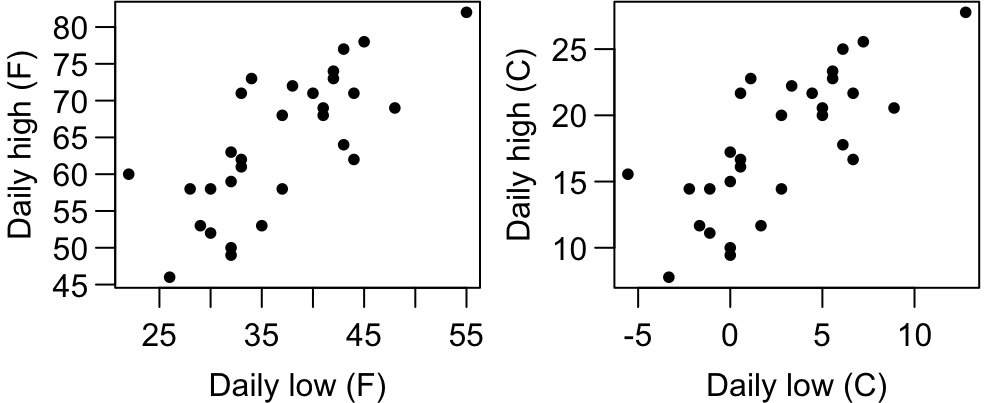
\includegraphics[width=0.8\linewidth]{ch09_24spr_files/figure-beamer/DailyHLFC-1} \end{center}

Are the correlation coefficients the same, or different? \newline
\hid{2-}{The same, both $r = 0.74$. Why?}
\end{frame}

\begin{frame}{}
\protect\hypertarget{section}{}
To see why, we are going to consider the effect of

\begin{itemize}
\item \textbf{translation} (adding the same number to each value of a variable),
\item \textbf{scaling} (multiplying each value of a variable by the same positive number), and
\item \textbf{reflection} (changing the sign of each value of a variable)
\end{itemize}

on the correlation coefficient.\bigskip

First we need to consider the effect of translation and scaling on
standard units.
\end{frame}

\begin{frame}{}
\protect\hypertarget{section-1}{}
\underline{Recall} Standard units are deviations from the average,
expressed in units of the SD. \vspace{-18pt}

\begin{center}
\includegraphics[width=0.9\linewidth]{ch09_24spr_files/figure-beamer/unnamed-chunk-1-1} \end{center}

When you shift all the entries on a list by some number,

\begin{itemize}
\tightlist
\item
  the average \((\bar{x})\) \hid{2-}{shifts by that number,}
\item
  the deviations from average (\(x_i-\bar{x}\)) \hid{3-}{don't change,}
\item
  the SD \hid{4-}{doesn't change}, and
\item
  the \textit{standard units \hid{5-}{don't change}.}
\end{itemize}
\end{frame}

\begin{frame}{}
\protect\hypertarget{section-2}{}
\begin{center}
\includegraphics[width=1\linewidth]{ch09_24spr_files/figure-beamer/unnamed-chunk-2-1} \end{center}

When all the entries on a list are multiplied by some number \(>0\),

\begin{itemize}
\tightlist
\item
  the average \((\bar{x})\) \hid{2-}{gets scaled by that number,}
\item
  the deviations from average (\(x_i-\bar{x}\)) \hid{3-}{get scaled,}
\item
  the SD \hid{4-}{gets scaled}, but
\item
  the \textit{standard units \hid{5-}{don't change}.}
\end{itemize}
\end{frame}

\begin{frame}{\red{Translation} and \red{Scaling} Have \red {no} Effect
on the Correlation}
\protect\hypertarget{and-have-effect-on-the-correlation}{}
since the correlation \(r\) between two variables \(x\) and \(y\) is
computed from the formula
\[r = \text{average of }(x\text{ in standard units}) \times
(y\text{ in standard units}).\]
\textbf{No matter how often you translate and scale $x$ and $y$,
the standard units won't change, and neither will $r$.}

\bigskip

\underline{Example}:\newline The correlation between two sets of
temperatures doesn't depend on whether the temperatures are measured in
Fahrenheit or centigrade.

\begin{itemize}
\tightlist
\item
  Converting from Fahrenheit to centigrade involves a translation
  (subtract 32) followed by a scaling (multiply by 5/9).
\end{itemize}
\end{frame}

\begin{frame}{Example}
\protect\hypertarget{example}{}
Suppose 2 datasets are generated for cars of some brand:

\begin{itemize}
\item[A.] Number of miles a car can drive using
one gallon of gas \textit{vs} speed of \underline{head wind}, in miles/hour;
\smallskip

\item[B.] Number of kilometers a car can drive using
one liter of gas \textit{vs} speed of \underline{head wind}, in km/hour;

\end{itemize}
\medskip

Do \(x\) (distance) and \(y\) (wind speed) have the same correlation
coefficient for these 2 datasets?

\medskip

\[\hid{2-}{r_A = r_B}\]
\end{frame}

\begin{frame}{}
\protect\hypertarget{section-3}{}
\alert{Watch out} --- if you multiply all the values of \textbf{ONE} of
the variables by a \textbf{negative} number, you'll \textbf{change the
sign} of the correlation coefficient: \vspace{-16pt}

\begin{center}
\includegraphics[width=1\linewidth]{ch09_24spr_files/figure-beamer/unnamed-chunk-3-1} \end{center}

What if the values of \textbf{both} variables are multiplied by negative
numbers? \hid{2-}{$r$ stay unchanged}
\end{frame}

\begin{frame}{Correlation Does Not Distinguish X \& Y}
\protect\hypertarget{correlation-does-not-distinguish-x-y}{}
Q: Is the correlation between \(x\) and \(y\) the same as the
correlation between \(y\) and \(x\)?

\begin{center}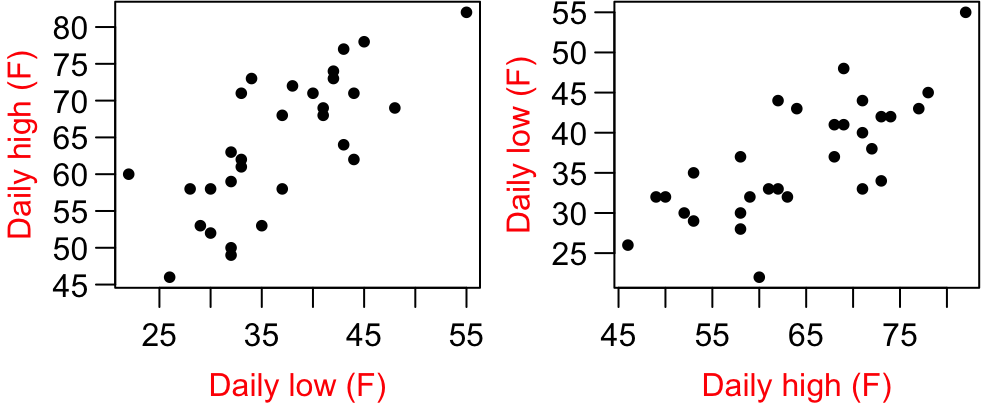
\includegraphics[width=1\linewidth]{ch09_24spr_files/figure-beamer/DailyHL-1} \end{center}

A: The two correlations are \textbf{the same}. Why?
\end{frame}

\begin{frame}{}
\protect\hypertarget{section-4}{}
Reason: The correlation between \(x\) and \(y\) involves averaging the
products
\[\text{($x$ in standard units) $\times$ ($y$ in standard units),\ while}\]
the correlation between \(y\) and \(x\) involves averaging the products
\[\text{($y$ in standard units) $\times$ ($x$ in standard units).}\] But
the order of the multiplications doesn't matter.

For example, if for some data point \(x\) is 3\textasciitilde SDs above
average and \(y\) is 2\textasciitilde SDs below average, then
\begin{align*}
&\text{($x$ in standard units) $\times$ ($y$ in standard units)}\cr
&= 3\times -2= -6 = -2 \times 3\cr
&= \text{($y$ in standard units) $\times$ ($x$ in standard units).}
\end{align*}

\textbf{Switching the axes has no effect on the correlation coefficient.}
\end{frame}

\begin{frame}{}
\protect\hypertarget{section-5}{}
\vspace{-10pt}
\linespread{0.9}
\begin{center}
\begin{tabular}{@{}c|cccc@{}}
       & Shifting & Scaling & Reflection & Sensitive \\[-2pt]
       & $x_i\rightarrow x_i+b$ & $x_i\rightarrow ax_i$ & $x_i\rightarrow -x_i$ & to extreme \\[-2pt]
       & for all $i$ & for all $i$ & for all $i$ & values?\\
\hline
Average   & shifted by $b$ & scaled by $a$ & change sign & Yes\\[-2pt]
$\bar{x}$ & $\bar{x}\rightarrow \bar{x}+b$ & $\bar{x}\rightarrow a\bar{x}$ &$\bar{x}\rightarrow -\bar{x}$ &\\
\hline
Median & shifted by $b$ & scaled by $a$ & change sign & No\\
\hline
SD     & unchanged      & scaled by $|a|$ & unchanged & Yes\\[-2pt]
       &                & SD $\rightarrow |a|\times\,$SD&&\\
\hline
IQR     & unchanged      & scaled by $|a|$ & unchanged & No\\[-2pt]
        &                & IQR $\rightarrow |a|\times\,$IQR&&\\
\hline
Standard& unchanged      & multiplied by & change sign & Yes\\[-2pt]
Units   &                & the sign of $a$ & &\\
\end{tabular}\end{center}
\smallskip

Let \(r(x,y)\) be the correlation coefficient of two variables \(x\) and
\(y\). \begin{align*}
r(x+a, y)&=r(x,y)\\
r(ax,y)&=\displaystyle\begin{cases}
 r(x,y)  & \text{if }a>0\\
 -r(x,y) & \text{if }a<0
\end{cases}\\
r(y,x)&= r(x,y)
\end{align*}
\end{frame}

\begin{frame}{Exercise: Correlation}
\protect\hypertarget{exercise-correlation}{}
Six data sets are shown below. The correlation is 0.8571 for (i), and
0.7857 for (ii). Can you find the correlations for (iii)(iv)(v)(vi)?

\begin{flushleft}
\small\tabcolsep=5pt
\begin{tabular}{rccccccccccccccccc}
&
\multicolumn{2}{c}{(i)}  &&
\multicolumn{2}{c}{(ii)} &&
\multicolumn{2}{c}{(iii)}&&
\multicolumn{2}{c}{(iv)} &&
\multicolumn{2}{c}{(v)}  &&
\multicolumn{2}{c}{(vi)} \\
& $x$ & $y$ && $x$ & $y$ && $x$ & $y$ &&  $x$ & $y$ && $x$ & $y$ && $x$ & $y$\\
\cline{2-3}\cline{5-6}\cline{8-9}\cline{11-12}\cline{14-15}\cline{17-18}
& 1 & 2 && 1 & 2 && 2 & 1 && 2 & 2 && 1 & ~4 && 0 & 1\\
& 2 & 3 && 2 & 3 && 3 & 2 && 3 & 3 && 2 & ~6 && 1 & 2\\
& 3 & 1 && 3 & 1 && 1 & 3 && 4 & 1 && 3 & ~2 && 2 & 3\\
& 4 & 4 && 4 & 4 && 4 & 4 && 5 & 4 && 4 & ~8 && 3 & 4\\
& 5 & 6 && 5 & 6 && 6 & 5 && 6 & 6 && 5 & 12 && 4 & 5\\
& 6 & 5 && 6 & 7 && 7 & 6 && 7 & 5 && 6 & 10 && 5 & 6\\
& 7 & 7 && 7 & 5 && 5 & 7 && 8 & 7 && 7 & 14 && 6 & 7\\
\cline{2-3}\cline{5-6}\cline{8-9}\cline{11-12}\cline{14-15}\cline{17-18}
$r=$ &
\multicolumn{2}{c}{0.8571}  &&
\multicolumn{2}{c}{0.7857}  &&
\multicolumn{2}{c}{\hid{2-}{0.7857}}&&
\multicolumn{2}{c}{\hid{3-}{0.8571}}&&
\multicolumn{2}{c}{\hid{4-}{0.8571}}&&
\multicolumn{2}{c}{\hid{5-}{1.0}}\\
\cline{2-3}\cline{5-6}\cline{8-9}\cline{11-12}\cline{14-15}\cline{17-18}
\end{tabular}
\end{flushleft}

\only<2>{\alert{(iii) is the same as (ii), with $x$ and $y$ switched, so $r$ remains the same as (ii), 0.7857.}}
\only<3>{\alert{(iv) comes from (i), by adding 1 to each $x$-value, so $r$ is the same as (i), 0.8751.}}
\only<4>{\alert{(v) comes from (i), by doubling each $y$-value, so $r$ is the same as (i), 0.8751.}}
\only<5>{\alert{$x$ and $y$ in (vi) has a perfect linear relationship, $y=x+1$. So $r=1$.}}
\end{frame}

\begin{frame}{Correlation Doesn't Reflect Strength of Nonlinear
Relations}
\protect\hypertarget{correlation-doesnt-reflect-strength-of-nonlinear-relations}{}
Both scatter plots below show \red{perfect nonlinear}
relations.\newline  All points fall on the quadratic curve
\(y = 2-x^2/2\).

\only<1| handout:0>{


\begin{center}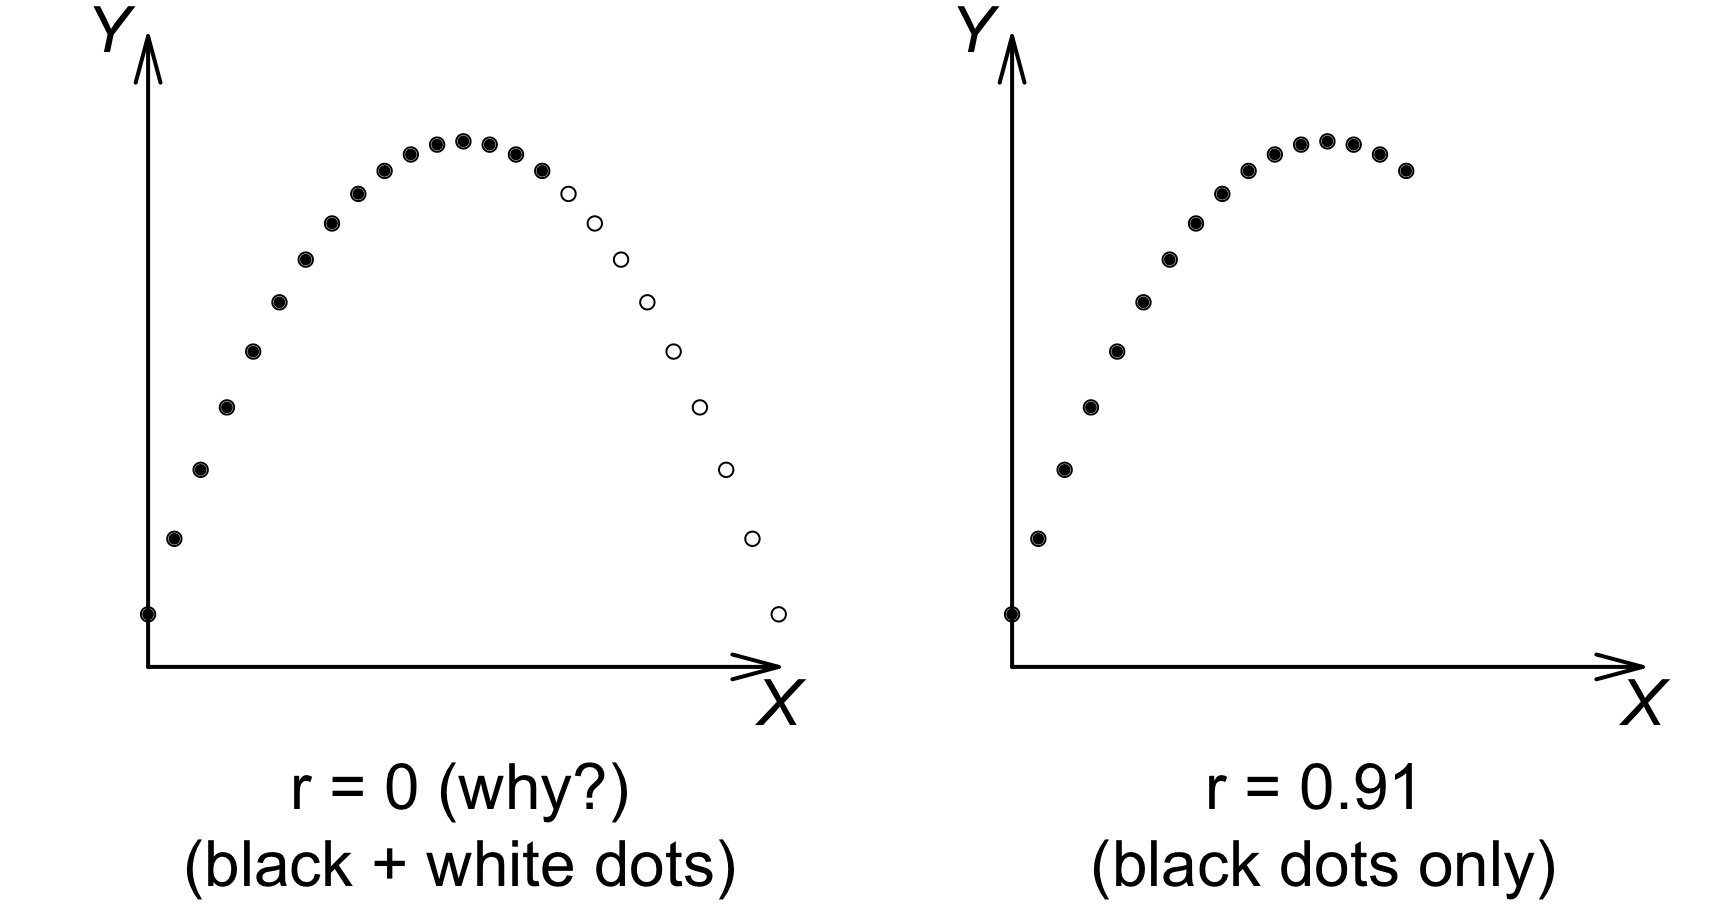
\includegraphics[width=0.9\linewidth]{ch09_24spr_files/figure-beamer/CovNonlinear-1} \end{center}


}\only<2| handout:1>{


\begin{center}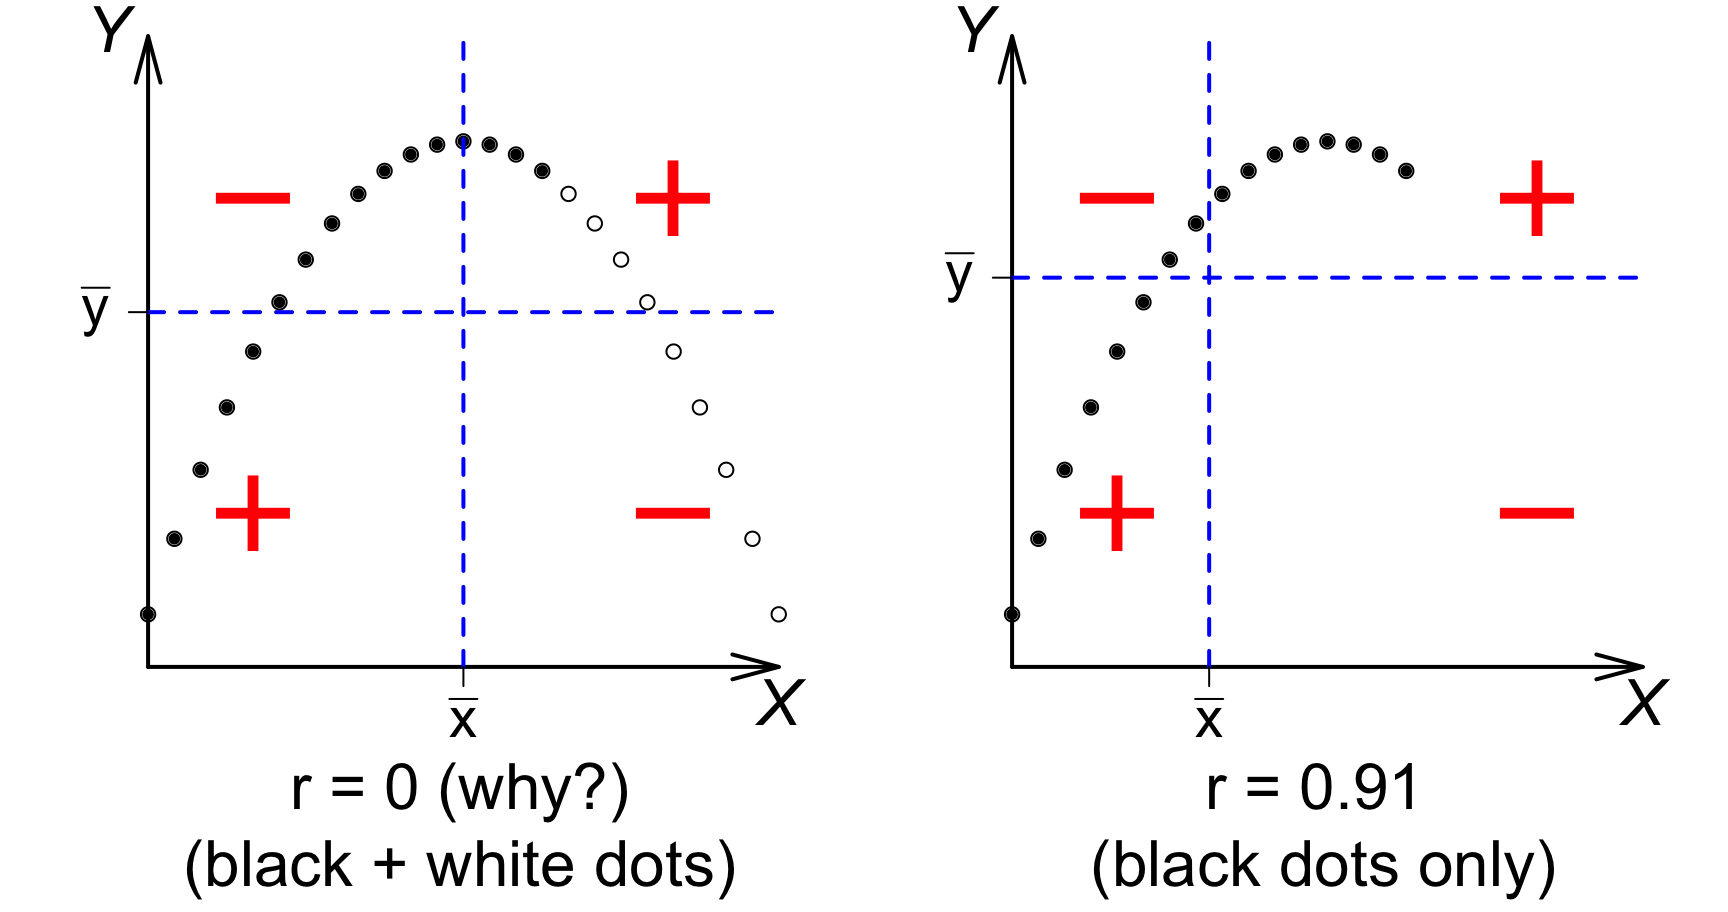
\includegraphics[width=0.9\linewidth]{ch09_24spr_files/figure-beamer/CovNonlinear-2} \end{center}


}
\pause

No matter how strong the relation, \(r\) is never 1 or \(-1\) if it's
nonlinear.\newline \(r\) can even be 0, like the plot above.
\end{frame}

\begin{frame}{Correlation Is VERY Sensitive to Outliers}
\protect\hypertarget{correlation-is-very-sensitive-to-outliers}{}
\begin{flushright}
\footnotesize
\begin{tabular}{rr}
$x$&$y$\\\hline
 3 & 10\\[-1pt]
11 & 11\\[-1pt]
40 &  5\\[-1pt]
17 & 19\\[-1pt]
12 & 19\\[-1pt]
 7 & 22\\[-1pt]
14 & 25\\[-1pt]
27 & 27\\[-1pt]
19 & 30\\[-1pt]
25 & 35\\[-1pt]
16 & 37
\end{tabular}
\end{flushright}

\normalsize
\vspace{-2in}

Sometimes a single outlier can change \(r\) drastically.\medskip

\vspace{-6pt}

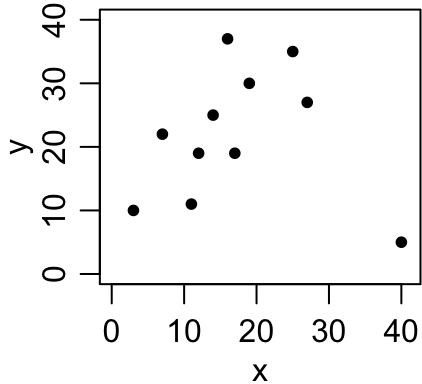
\includegraphics[width=0.35\linewidth]{ch09_24spr_files/figure-beamer/outlier-1}

With the outlier \((40,5)\), the correlation is \(r=0.0044\).\newline
Removing the outlier, the correlaiton becomes \(r=0.691\).
\end{frame}

\begin{frame}{When Data Points Are Clustered \ldots{}}
\protect\hypertarget{when-data-points-are-clustered}{}
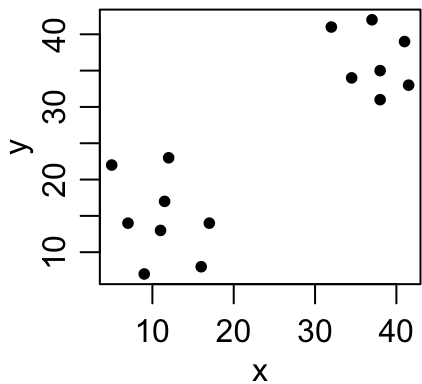
\includegraphics[width=0.4\linewidth]{ch09_24spr_files/figure-beamer/clustered-1}

\vspace{-1.4in}
\begin{flushright}
\begin{minipage}{0.55\textwidth}
In the plot above, each of the two clusters exhibits a weak negative association  ($r=-0.336$ and $-0.323$).
\par\medskip

But the whole diagram shows a moderately strong positive association ($r=0.849$).
\end{minipage}
\end{flushright}
\bigskip

\begin{itemize}
\tightlist
\item
  This is an example of the \textbf{Simpson's paradox}.
\item
  An overall \(r\) can be misleading when data points are clustered.
\item
  Cluster-wise \(r\)'s should be reported as well.
\end{itemize}
\end{frame}

\begin{frame}[fragile]{Example: Auto Data}
\protect\hypertarget{example-auto-data}{}
Auto is a data set containing information about 392 car models in the
1980s. The variables include

\begin{itemize}
\tightlist
\item
  \texttt{acceleration}: Time to accelerate from 0 to 60 mph (in
  seconds)
\item
  \texttt{horsepower}: Engine horsepower
\item
  \texttt{weight}: Vehicle weight (lbs.)
\end{itemize}
\end{frame}

\begin{frame}[fragile]{Example: Auto Data (2)}
\protect\hypertarget{example-auto-data-2}{}
\begin{center}
\includegraphics[width=0.5\linewidth]{ch09_24spr_files/figure-beamer/unnamed-chunk-6-1} \end{center}

From the scatter plot, \texttt{weight} and \texttt{acceleration} are
negatively correlated. Is that reasonable?
\end{frame}

\begin{frame}[fragile]{Example: Auto Data (3)}
\protect\hypertarget{example-auto-data-3}{}
\begin{center}
\includegraphics[width=0.7\linewidth]{ch09_24spr_files/figure-beamer/unnamed-chunk-7-1} \end{center}

Consider car models of similar \texttt{horsepower}, are \texttt{weight}
and \texttt{acceleration} positively or negatively correlated?
\end{frame}

\begin{frame}{Example: Auto Data (4)}
\protect\hypertarget{example-auto-data-4}{}

\includegraphics{ch09_24spr_files/figure-beamer/unnamed-chunk-9-1.png}
\end{frame}

\begin{frame}{Correlation Indicates Association, \textit{Not} Causation}
\protect\hypertarget{correlation-indicates-association-causation}{}
\begin{center}
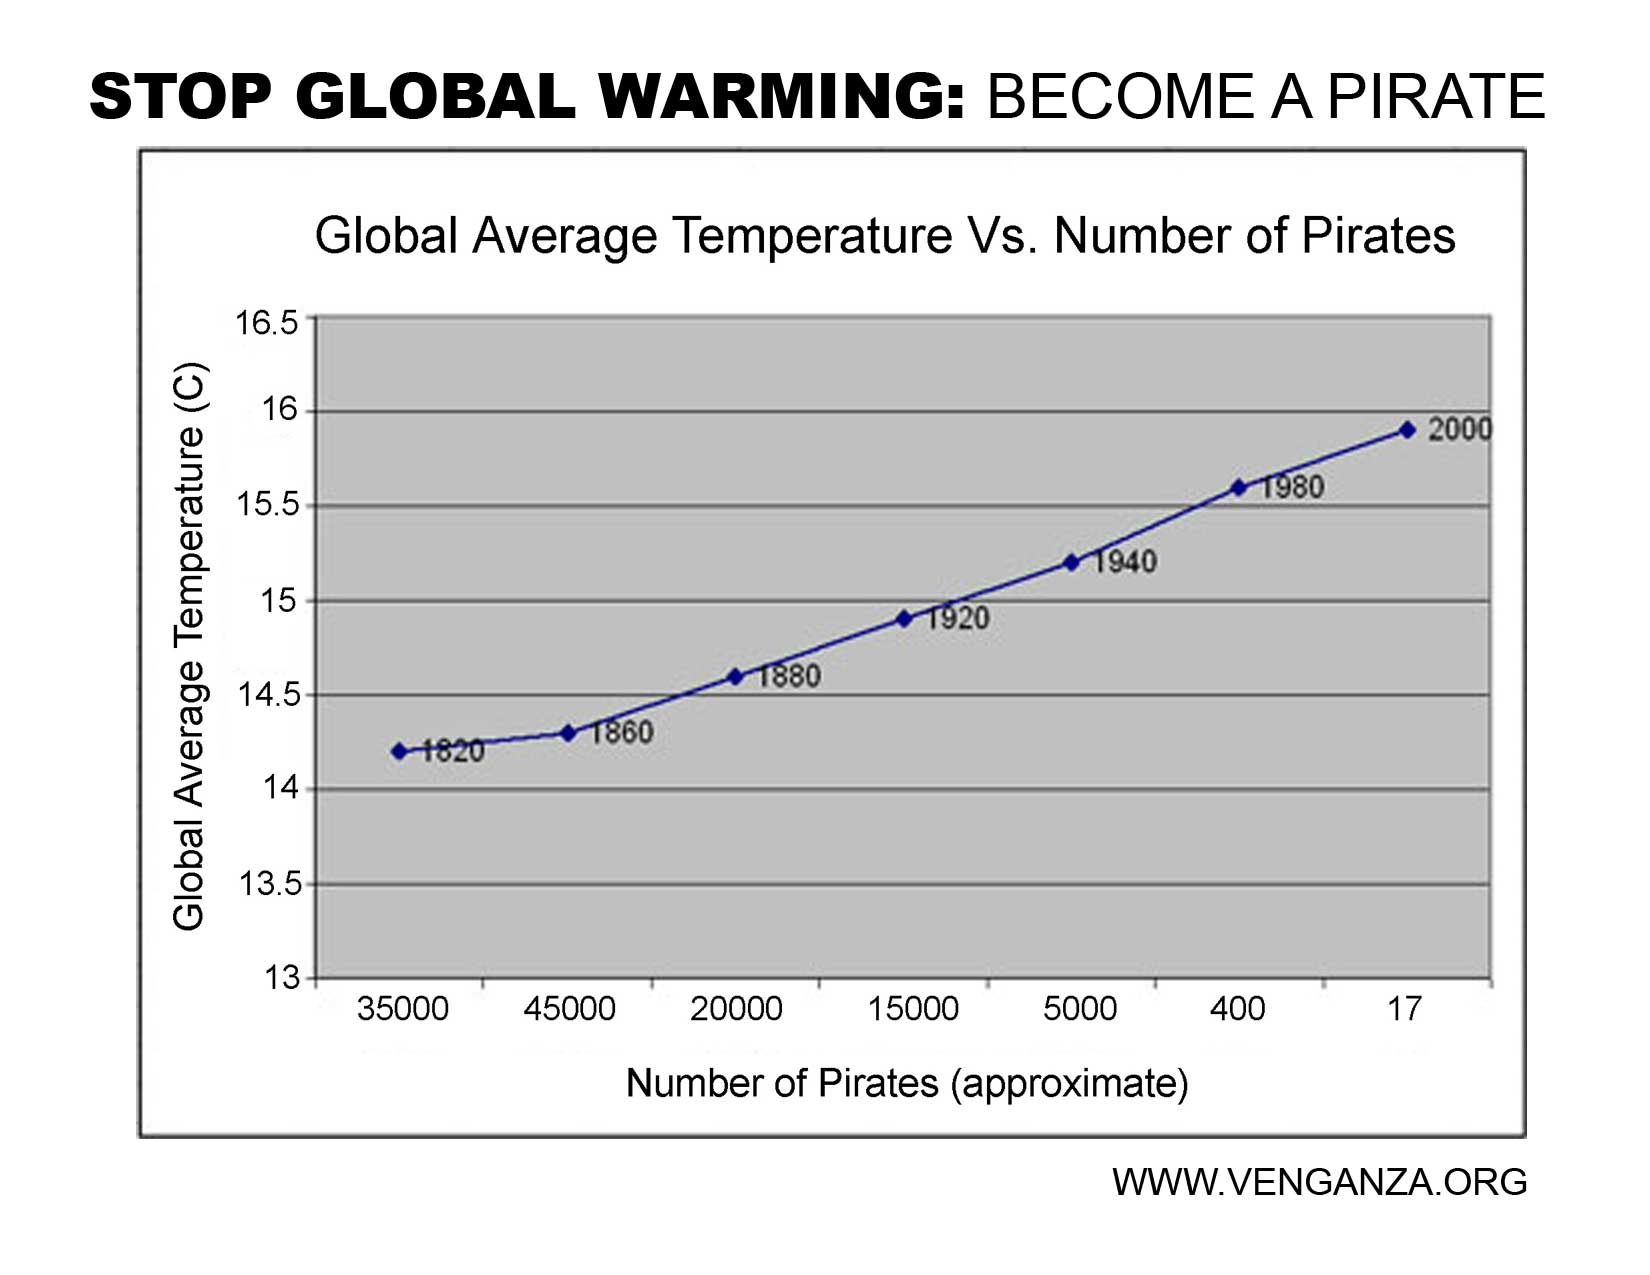
\includegraphics[width=\textwidth]{./C09/Pirate.jpg}
\end{center}
\end{frame}

\begin{frame}{Always Check the Scatter Plots (1)}
\protect\hypertarget{always-check-the-scatter-plots-1}{}
The 4 data sets below have identical \(\overline{x}\), \(\overline{y}\),
\(s_x\), \(s_y\), and \(r\).

\begin{center}
\tabcolsep=4pt
\small\renewcommand{\arraystretch}{0.9}
\begin{tabular}{c|cc|cc|cc|cc}
& \multicolumn{2}{c}{Dataset 1}
& \multicolumn{2}{c}{Dataset 2}
& \multicolumn{2}{c}{Dataset 3}
& \multicolumn{2}{c}{Dataset 4}\\[-3pt]
& $x$ & $y$ & $x$ & $y$ & $x$ & $y$ & $x$ & $y$\\\hline
&10 & ~8.04 & 10 & 9.14 & 10 & ~7.46 & ~8 & ~6.58 \\
&~8 & ~6.96 & ~8 & 8.14 & ~8 & ~6.77 & ~8 & ~5.76 \\
&13 & ~7.58 & 13 & 8.75 & 13 & 12.76 & ~8 & ~7.71 \\
&~9 & ~8.81 & ~9 & 8.77 & ~9 & ~7.11 & ~8 & ~8.84 \\
&11 & ~8.33 & 11 & 9.26 & 11 & ~7.81 & ~8 & ~8.47 \\
&14 & ~9.96 & 14 & 8.10 & 14 & ~8.84 & ~8 & ~7.04 \\
&~6 & ~7.24 & ~6 & 6.13 & ~6 & ~6.08 & ~8 & ~5.25 \\
&~4 & ~4.26 & ~4 & 3.10 & ~4 & ~5.36 & 19 & 12.50 \\
&12 & 10.84 & 12 & 9.13 & 12 & ~8.15 & ~8 & ~5.56 \\
&~7 & ~4.82 & ~7 & 7.26 & ~7 & ~6.42 & ~8 & ~7.91 \\
&~5 & ~5.68 & ~5 & 4.74 & ~5 & ~5.73 & ~8 & ~6.89 \\\hline
Ave & 9    & 7.5  & 9    & 7.5  & 9    & 7.5  & 9    & 7.5   \\
SD  & 3.16 & 1.94 & 3.16 & 1.94 & 3.16 & 1.94 & 3.16 & 1.94  \\
$r$
& \multicolumn{2}{c}{0.82}
& \multicolumn{2}{c}{0.82}
& \multicolumn{2}{c}{0.82}
& \multicolumn{2}{c}{0.82}
\end{tabular}
\normalsize
\end{center}
\end{frame}

\begin{frame}{Always Check the Scatter Plots (2)}
\protect\hypertarget{always-check-the-scatter-plots-2}{}
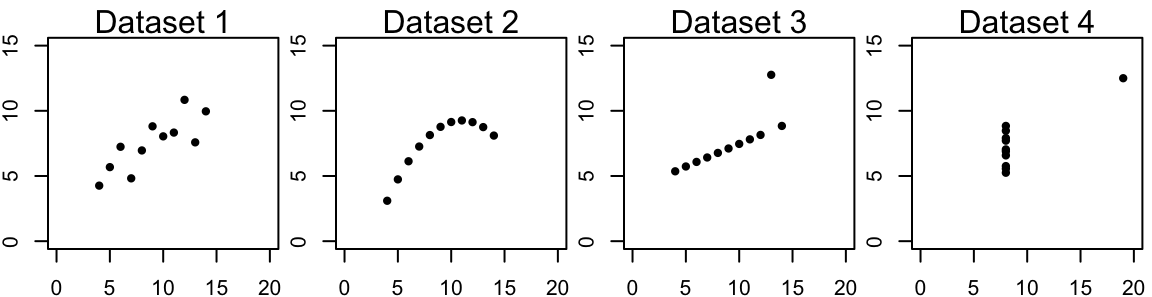
\includegraphics[width=1\linewidth]{ch09_24spr_files/figure-beamer/4datasets-1}

\begin{itemize}
\tightlist
\item
  For Dataset 2, \(y\) can be predicted exactly
  from\textasciitilde{}\(x\). But \(r < 1\), because \(r\) only measures
  \textbf{linear} association.
\item
  For Dataset 3, \(r\) would be 1 instead of 0.82 if the outlier were
  actually on the line. \medskip
\end{itemize}

The correlation coefficient can be misleading in the presence of
outliers, multiple clusters, or nonlinear association.
\end{frame}

\begin{frame}{Ecological Correlations}
\protect\hypertarget{ecological-correlations}{}
For each of 3 geographical regions in the U.S., a political scientist
computes the average income and average educational level for the men
aged 25--64 living in those regions. The correlation between regional
average education and regional average income is 0.9. Does this give a
fair estimate of the strength of the association between education and
income for the men being studied?

\begin{center}
\includegraphics[width=0.8\linewidth]{ch09_24spr_files/figure-beamer/unnamed-chunk-10-1} \end{center}

\begin{itemize}
\tightlist
\item
  No.~Taking averages eliminates spread, and gives a misleading
  impression of tight clustering.
\end{itemize}
\end{frame}

\begin{frame}{Ecological Correlations (Cont'd)}
\protect\hypertarget{ecological-correlations-contd}{}
In general, given a dataset of pairs of \(x\) and \(y\) values, divide
the dataset into subgroups, and take the averages of \(x\) and \(y\)
values within each subgroup. The correlation of \(x\)-average and
\(y\)-average across the subgroups is \textbf{ecological correlation}.\\
(\textit{Note}: this is different from correlation among variables from
a population comprised of distinct clusters.)

\bigskip

\hl{Ecological correlations}, which are based on rates or averages, tend
to overstate the strength of associations.
\end{frame}

\begin{frame}{Summary}
\protect\hypertarget{summary}{}
\linespread{1.1}
\begin{itemize}
\item The correlation coefficient is a pure number, without units. It is not affected by:
\begin{itemize}\normalsize
\item interchanging the two variables;
\item adding the same number to all the values of one variable;
\item multiplying all the values of one variable by the same positive
number.
\end{itemize}

\item The correlation coefficient can be misleading in the presence of
outliers or nonlinear association. Whenever possible, look at the
scatter diagram to check for these problems.

\item \textbf{Ecological correlations}, which are based on rates or averages,
tend to overstate the strength of associations.

\item Correlation measures association. But association does not necessarily
show causation. It may only show that both variables are simultaneously
influenced by some 3rd variable.
\end{itemize}
\end{frame}

\end{document}
